\chapter{实数}
实数是现实世界中最基本的数系,我们采用逼近法来研
究实数,逼近法是一种原理简朴但是应用广泛的方法,它将
贯穿于本书的微积分学部分,是一支主力军。

\section{度量与实数}

一般说来,常见的量可以归纳成两类:比如一堆蛋,
一群牛,它们都具有天然的个别单元,对它们的处理方法是
数一数它们的个数,用来数个数的数学体系就是“自然数系”。
另一类量如长度、重量、温度、压力这种量不具有天然不可
分割的单元!我们处理这类量的办法是度量,由度量产生的
数系就是“实数系”,换句话说,实数系乃是将常见的长度、
重量等这一类量的通性加以抽象化、组织化所得出来的数学
体系,它是用来表达、计算这一类连续变化的量的简洁、有
效工具。

下面将以长度为例,说明度量和实数的起源。

\subsection{长度的度量}
因为长度这种量并不是有天然不可分割的单位,所以我
们只好选用人为的单位长,设线段
$u$是所选用的单位长,当
我们要度量一个线段$a$时,我们所要去求的乃是$a$与$u$之间的
“比值”,这个比值是一个实数$k$, 我们就说线段$a$的长度是
$k$单位,现在让我们耐心地分析一下,在实践中这个“比
值”是怎样求得的?

我们先拿一根尺$u$, 用它 
去逐段比量线段$a$, 假如$a$恰好是$n$个和$u$等长的线段首尾连接
而成,我们说$u$恰好整量$a$, $a$的长度是$n$单位,但是假如$u$
不能整量$a$,例如在图6.1中的线段,$a$比$4u$要长些,却比$5u$要
短些。

\begin{figure}[htp]
    \centering
\begin{tikzpicture}
\draw (0,1)--node[above]{$u$}(1,1);
\foreach \x in {0,1}
{
    \draw (\x,1)--(\x,1.1);
}
\draw (0,0)--node[above=5pt]{$a$}(4.75,0);
\foreach \x in {0,1,...,4,4.25,4.5,4.75}
{
    \draw (\x,0)--(\x,0.1);
}
\end{tikzpicture}
    \caption{}
\end{figure}


试着去解决上述不能整量的矛盾的一个简朴想法是:把
单位长$u$适当地加以等分,希望分后的“分单位”能够整量
$a$(比如上面的例子中,$\frac{1}{4}u$
就可以整量$a$, 即$a=4\frac{3}{4}u=\frac{19}{4}u$),一般地,假如$a$
能用$\frac{1}{m}u$这个分单位整量,譬如$a=\frac{n}{m}u$,则$a,u$之间的比值是个有理数(也称为比数)。在
这儿,就自然地产生下述基本问题。

\textbf{度量基本问题 } 任给两个量$a,b$之间的比值是否一定是
个有理数(比数)?换句话说,对于任给两个量$a,b$是否存
在一个同时整量$a,b$的$u$?

上面这个问题的重要性可以分别从正、反两面来分析:
假如任何两个量的比值总是有理数,那么有理数全体就足够
处理度量问题,这样度量问题就变得十分简单了。从另一方
面来看,假如两个量之间的比值不一定是有理数,则有理数
全体(简称有理数系或比数系)就不足以处理度量问题,换
句话说,我们就得学会一个不只包含有理数系的实数系,才
能充分处理度量问题。总之,上述基本问题是必须实事求是
地弄明白的!

\subsection{无理数(非比实数)的存在}
不难给出,两个线段的比值不可能是有理数的一个简单
例子,如图6.2所示,各边为单位长
度的正方形的对角线$\ell$与边长之比就
不能是个有理数。
\begin{figure}[htp]
    \centering
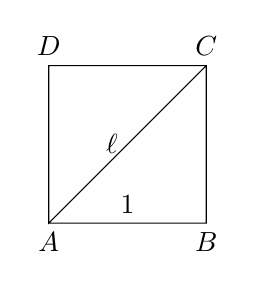
\begin{tikzpicture}
\draw (0,0)node[below]{$A$} --node[above]{1}(2,0)node[below]{$B$}-- (2,2)node[above]{$C$}--(0,2)node[above]{$D$}--(0,0)--node[left]{$\ell$}(2,2);
\end{tikzpicture}
    \caption{}
\end{figure}

因为根据勾股定理,
$\ell^2=2$, 所以,如果$\ell$是个有理数,设其等于
$\frac{p}{q}$,这里$q$和$p$是两个互质的正整
数,我们将有
\[p^2=2q^2\]
根据上述方程,$p$是偶数,因此$p$本身也必定是偶数,譬如
说,$p=2p'$, 用$2p'$代替$p$, 我们得到
\[4({p'}^2)=2q^2\]
或者,
\[q^2=2(p')^2\]
因而$q^2$是偶数,于是$q$也是偶数,然而这同我们所作的$p$和$q$没
有公因子的约定相矛盾,这一矛盾是由假设对角线长能够表
示为既约分数$\frac{p}{q}$
引起的,所以这一假设是错误的。

这一用反证法推导的例子,表明符号$\sqrt{2}$不能对应于任
何有理数。另一例子是$\pi$——圆的周长与直径的比,证明$\pi$
不是有理数要复杂得多,并且直到近代才做到。不属于有理
数系的实数有很多,所以在某种意义上远比有理数更为普
遍,因此,从几何度量的客观实际需要出发,我们不得不增
添一类新数,这一类新数叫\textbf{无理数}。有理数和无理数的全体
统称为\textbf{实数系}。当我们面对着实数系中还存在着许多“无理
数”这一事实时,怎样去有系统地学习实数系的性质并充分
掌握其用法,这便成为我们的一个迫切的基本课题。下面所
要谈的逼近法,就是一种有效地利用熟知的有理数系作为桥
梁,向实数系进军的捷径。

\subsection{逼近法}
通过已知的有理数系去了解实数系的可能性基于下述基
本事实,那就是:任何无理数都可以用有理数去逼近它!
现在我们用数轴来图解有理数系与实数系间的关系。如图6.3
所示。

\begin{figure}[htp]
    \centering
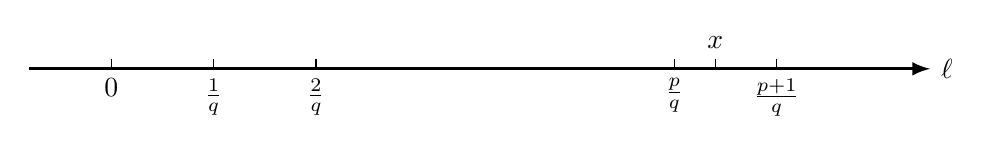
\begin{tikzpicture}[>=latex, scale=1.3]
\draw[very thick, ->] (-0.8,0)--(8,0)node[right]{$\ell$};
\foreach \x/\xtext in {0/0,1/\frac{1}{q},2/\frac{2}{q},5.5/\frac{p}{q},6.5/\frac{p+1}{q}}
{
    \draw (\x, 0)node[below]{$\xtext$}--(\x,.1);
} 
\draw (5.9,0)--(5.9,.1)node[above]{$x$};

\end{tikzpicture}
    \caption{}
\end{figure}

在上面坐标系中,所有以整数为坐标的点,在直线$\ell$上
成一均匀分布的点集,其相邻两点间的距离都是1单位;同
样的,所有坐标是$\frac{p}{2}$, $(p=0,\pm1,\pm2,\ldots)$
的点,在直线上
成一均匀分布的点集,其相邻两点间的距离都是$\frac{1}{2}$
单位;设$q$为一指定的自然数,则所有坐标是$\frac{p}{q},\; p\in\mathbb{Z}$的点在直线
上成一均匀分布的点集,其相邻两点间的距离是$\frac{1}{q}$
单位。只
要将$q$取成足够大的自然数,则能使数$\frac{1}{q}$
想要多么小就可
以多么小。这个现象说明在直线上任何一段很短的线段中,
都有坐标是有理数的点,也就是任何两个有理数点之间都有
有理数点,这就是\textbf{有理数点集稠密性},但是这个现象并不表
示有理点就可以填满整个直线,例如长度为$\sqrt{2}$, $\sqrt{3}$的线
段,若将它的一个端点放在数轴的原点,则另一端点在直线
的坐标就不是有理数。现在我们的问题是如何说明实数同原
来熟悉的有理数,因而最终同整数的关系。让我们再回到图
6.3的数轴$\ell$上,显然$\ell$上面的每一个点或者是坐标
为$\frac{p}{q}$的有理点,或者处于两个相邻的有理点
$\frac{p}{q}$和$\frac{p+1}{q}$
之间,换言之,给了任何自然数$q$之后,对于每一个实数$x$, 一定有一整
数$p$, 使得
\[\frac{p}{q}\le x<\frac{p+1}{q}\]
即
\[\frac{p}{q}\le x<\frac{p}{q}+\frac{1}{q}\]
从这三个数各减去$\frac{p}{q}$,得到
\[0\le x-\frac{p}{q}<\frac{1}{q}\]
于是
\[\left|x-\frac{p}{q}\right|<\frac{1}{q}\]
这个不等式说明,只要将$q$取成足够大的自然数,每一个实数$x$
与有理数$\frac{p}{q}$
的误差想要多么小就可以多么小。

下面我们来说明每一个无理数如何通过越来越逼近它的
有理数数列来描述它。

\subsubsection{二分逼近法}

现在让我们用二分逼近法来说明任何无理
数都可以用有理数数列去逼近它,使得误差小到任意小。

设某无理数$x$位于线段$A_0B_0=[a_0,b_0]$内(亦即$a_0<x<b_0$,
$a_0$, $b_0$均为有理数),见图6.4。

\begin{figure}[htp]
    \centering
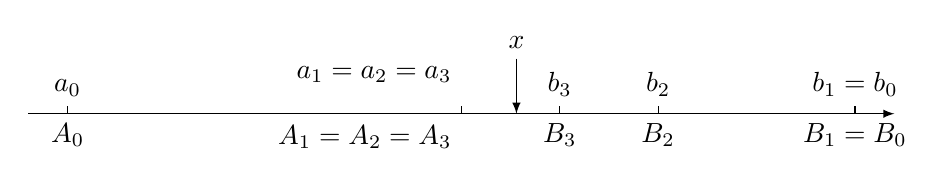
\begin{tikzpicture}[>=latex]
\draw[->] (-0.5,0)--(10.5,0);
\foreach \x/\xtext in {0/a_0,10/b_1=b_0,7.5/b_2,6.25/b_3}
{
    \draw (\x,0)--(\x,.1)node[above]{$\xtext$};
}  
\draw (5,0)--(5,.1);

\node at  (5,-.3)[left]{$A_1=A_2=A_3$};
\node at (6.25,0)[below]{$B_3$};
\node at (7.5,0)[below]{$B_2$};
\node at (0,0)[below]{$A_0$};
\node at (10,0)[below]{$B_1=B_0$};
\node at  (5,.5)[left]{$a_1=a_2=a_3$};
\draw[->] (5.7,.7)node[above]{$x$}--(5.7,0);
\end{tikzpicture}   
    \caption{}
\end{figure}

我们将线段$A_0B_0=[a_0,b_0]$等分为两段,亦即$\left[a_0,\frac{a_0+b_0}{2}\right]$和$\left[\frac{a_0+b_0}{2},b_0\right]$;而把$x$所在的那一段叫做$A_1B_1=[a_1,b_1]$, 换句话说,当$a_0<x<\frac{a_0+b_0}{2}$时,$a_1=a_0$, $b_1=\frac{a_0+b_0}{2}$;当$\frac{a_0+b_0}{2}<x<b_0$,$a_1=\frac{a_0+b_0}{2}$,$b_1=b_0$。这样逐
次二等分,由$A_1B_1$求得$A_2B_2$,……,由$A_{n-1}B_{n-1}$求得 $A_nB_n$,
永远无休止地二等分下去,因为每次二等分后,分段长度减
半,所以$x$所在的线段就可以小到任何需要的程度。现在把
上面的二分逼近过程写下来,就得到$a_n,b_n,x$的下列关系:
\begin{enumerate}
    \item $A_0B_0=[a_0, b_0]\supseteq A_1B_1 =[a_1,b_1]
    \supseteq \cdots \supseteq A_nB_n=[a_n, b_n]\supseteq A_{n+1}B_{n+1}=[a_{n+1},b_{n+1}]\supseteq \cdots \supseteq \{x\}$,即:
\[a_0\le a_1\le a_2\le\cdots\le a_n\le \cdots <x<\cdots\le b_n\le\cdots\le b_2\le b_1\le b_0\]

\item $b_n-a_n=\frac{1}{2}(b_{n-1}-a_{n-1})=\cdots=\frac{1}{2^n}(b_0-a_0)$,这
就保证了$a_n$或$b_n$和$x$之间的误差小于$\frac{1}{2^n}(b_0-a_0)$, 即$|x-a_n|<\frac{1}{2^n}(b_0-a_0)$或$|x-b_n|<\frac{1}{2^n}(b_0-a_0)$, 只要$n$够大,上述误
差就可以小到任意小。
\item 实数$x$由它的夹逼数列:
\[a_0\le a_1\le a_2\le\cdots\le a_n\le \cdots <x<\cdots\le b_n\le\cdots\le b_2\le b_1\le b_0\]
其中:$b_n-a_n=\frac{1}{2^n}(b_0-a_0)$
唯一确定,即没有另一点能够处在
所有的线段$A_nB_n$之中。
\end{enumerate}

要证明这个数的唯一性,我们假定另有第二个数$y$也属
于一切线段$A_nB_n$之中,于是这些线段的每一个长$b_n-a_n$都应
不小于$|x-y|$, 但是,因为线段$A_nB_n$可以任意小,只要$n$足
够大,$A_nB_n$的长就会小于$x$和$y$之间的距离,这就得出矛盾。
所以实数$x$能由它的夹逼数列唯一确定。

现在以$x=\sqrt{2}$, $a_0=1$, $b_0=2$为例来说明如何用二分
逼近法求$\sqrt{2}$的近似值,如图6.5所示。
\begin{figure}[htp]
    \centering
\begin{tikzpicture}[>=latex]
    \draw[->] (-0.5,0)--(10.5,0);
\foreach \x /\xtext in {0/a_0=a_1=1,10/b_0=2,5/{},2.5/a_2,3.75/a_3=a_4, 4.375/{}}
{
    \draw(\x,0)--(\x,.1)node[above]{$\xtext$};
}

\draw[->] (4.14,-.7)node[below]{$\sqrt{2}$}--(4.14,0);

\node at (5,-0.3)[right]{$b_1=b_2=b_3$};
\node at (4.375,-0.3){$b_4$};
\end{tikzpicture}
    \caption{}
\end{figure}

\begin{enumerate}
    \item  $\frac{1}{2}\left(a_{0}+b_{0}\right)=\frac{3}{2},\qquad \left(-\frac{3}{2}\right)^{2}=\frac{9}{4}>2 \quad\Rightarrow\quad\frac{3}{2}>\sqrt{2}$
    
    故 $a_{0}=a_{1}=1,\qquad   b_{1}=\frac{3}{2}$

    \item   $\frac{1}{2}\left(a_{1}+b_{1}\right)=\frac{5}{4},\qquad \left(\frac{5}{4}\right)^{2}=\frac{25}{16}<2 \quad\Rightarrow\quad \frac{5}{4}<\sqrt{2}$
    
    故$a_{2}=\frac{5}{4}, \qquad  b_{2}=b_{1}=\frac{3}{2}$

    \item  $\frac{1}{2}\left(a_{2}+b_{2}\right)=\frac{11}{8},\qquad \left(\frac{11}{8}\right)^{2}=\frac{121}{64}<2 \quad\Rightarrow\quad \frac{11}{8}<\sqrt{2}$
    
    故 $a_{3}=\frac{11}{8},\qquad  b_{3}=b_{2}=\frac{3}{2}$

    \item   $\frac{1}{2}\left(a_{3}+b_{3}\right)=\frac{23}{16},\qquad \left(\frac{23}{16}\right)^{2}=\frac{529}{256}>2 \quad\Rightarrow\quad \frac{23}{16}>\sqrt{2}$
    
    故 $a_{4}=a_{3}=\frac{11}{8},\qquad  b_{4}=\frac{23}{16}$

    \item  $\frac{1}{2}\left(a_{4}+b_{4}\right)=\frac{45}{32},\quad \left(\frac{45}{32}\right)^{2}=\frac{2025}{1024}<2 \quad\Rightarrow\quad \frac{45}{32}<\sqrt{2}$
    
     故$a_{5}=\frac{45}{32}, \qquad b_{5}=b_{4}=\frac{23}{16}
    $
    
    \item  $\frac{1}{2}\left(a_{5}+b_{5}\right)=\frac{91}{64},\quad \left(\frac{91}{64}\right)^{2}=\frac{8281}{4096}>2 \quad\Rightarrow\quad \frac{91}{64}>\sqrt{2}$
    
     故$a_{6}=a_{5}=\frac{45}{32}, \qquad b_{6}=\frac{91}{64}
    $

    
    \item  $\frac{1}{2}\left(a_{6}+b_{6}\right)=\frac{181}{128},\quad \left(\frac{181}{128}\right)^{2}=\frac{32761}{16314}<2 \quad\Rightarrow\quad \frac{181}{128}<\sqrt{2}$
    
     故$a_{7}=\frac{181}{128}, \qquad b_{7}=b_{6}=\frac{91}{64}$,这时,$\frac{181}{128}<\sqrt{2}<\frac{91}{64}$,把$\frac{181}{128}$作为$\sqrt{2}$的不足近似值,其误差小于
$\frac{1}{2^7}=\frac{1}{128}$。
\end{enumerate}

照这样逐步计算,每次只要检验$\frac{1}{2}(a_{n-1}+b_{n-1})$的平方
和2之间的大小次序关系,就能确定
$\frac{1}{2}(a_{n-1}+b_{n-1})$应该是
$a_n$还是$b_n$, 显然的,这样所求得的$a_n,b_n$和$\sqrt{2}$有下列关系:
\[a_n<\sqrt{2}<b_n,\quad b_n-a_n=\frac{1}{2^n},\; (n=1,2,3,\ldots)\]

我们可以把$a_n$叫做$\sqrt{2}$的一个“$n$阶不足近似值”。$b_n$叫做$\sqrt{2}$的
一个“$n$阶过剩近似值”,它们和$\sqrt{2}$的差的绝对值小于
$\frac{1}{2^n}$。


\subsubsection{十分逼近法}

上面所讨论的二分逼近法只不过是逼近法
的一种,譬如,对于任何大于1的整数$q$, 我们可以仿照上
法用逐次$q$等分而得到“$q$分逼近法”,但是实用起来,$q$愈大
则每次要去确定$x$属于$q$个分段中的哪一段时所需做计算也就
愈繁,所以二分逼近法比较简便,再者,在$q$分逼近法中,
用来逼近的数$a_n,b_n$都是那些分母是$q$的方幂的分数;而常
用的“十进小数”也就是分母是10的方幂的分数,例如,
\[1.4=\frac{14}{10},\quad  1.41=\frac{141}{100}=\frac{141}{10^2},\quad \ldots \]
所以十分逼近法也就是用小数去逼近的方法,现在再以$\sqrt{2}$为例,简要地说明十分逼近法如下:

将线段$[1,2]$十等分,其分点分别是$1.1,1.2,\ldots,
1.9$, 看看哪些分点的平方小于2, 哪些大于2,算一下就
得出:

$(1.1)^2,(1.2)^2,(1.3)^2,(1.4)^2=1.96<2<2.25=
(1.5)^2,(1.6)^2,\ldots ,(1.9)^2$. 所以$1.4<\sqrt{2}<1.5$, $\sqrt{2}$属于
分段$[1.4,1.5]$;

再把$[1.4,1.5]$十等分,分点分别是$1.41,1.42,\ldots,
1.49$, 再算一下,由$(1.41)^2=1.9891<2<2.0164=
(1.42)^2,(1.43)^2,\ldots,(1.49)^2$, 就得出$\sqrt{2}$属于分段$[1.41,1.42]$, 再一次十等分,然后再由计算可以确定$\sqrt{2}$属于分
段$[1.414,1.415]$, 这样逐次十等分,就可以求得一个$n$位
小数$a_n$使得
\[a_n<\sqrt{2}<b_n=a_n+\left(\frac{1}{10}\right)^n\]

在实用时,我们按照实际问题所需要的精确度,求到足
够位数(即$\left(\frac{1}{10}\right)^n$小于许可误差)。这里我们用普通的算术
法则对2作开方运算将得到一个足够精确的小数。例如,
求$\sqrt{2}$的不足近似值和过剩近似值,精确到$\frac{1}{10^4}$。
计算如下:

\begin{center}
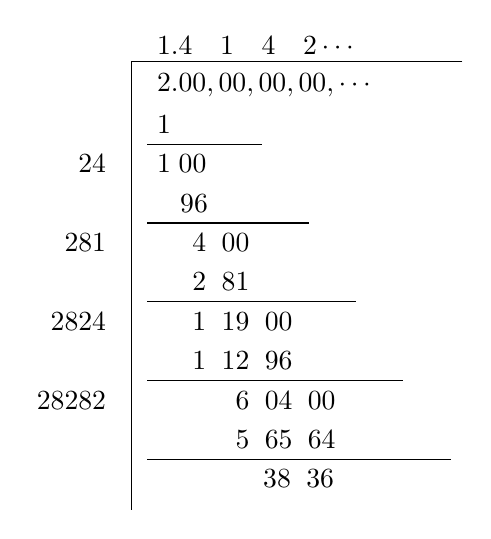
\begin{tikzpicture}[scale=2]
\node at (0,0)[right]{$\qquad \quad\;\;\;  38\;\;36$};
\node at (0,0.25)[right]{$\qquad\;\;\;  5\;\;65\;\;64$};
\node at (0,0.5)[right]{$\qquad \;\;\; 6\;\;04\;\;00$};
\node at (0,0.75)[right]{$\quad \; 1\;\;12\;\;96$};
\node at (0,1)[right]{$\quad \; 1\;\;19\;\;00$};
\node at (0,1.25)[right]{$\quad\; 2\;\;81$};
\node at (0,1.5)[right]{$\quad \; 4\;\;00$};
\node at (0,1.75)[right]{$\;\;\; 96$};
\node at (0,2)[right]{$1\;00$};
\node at (0,2.25)[right]{$1$};
\node at (0,2.5)[right]{$2.00,00,00,00,\cdots$};
\node at (0,2.75)[right]{$1.4\quad1\quad4\quad2\cdots$};
\draw(2,2.65)--(-0.1,2.65)--(-0.1,-.2);

\foreach \x/\xtext in {2/24,1.5/281,1/2824,.5/28282}
{
   \node at (-.2,\x)[left]{\xtext};
}

\foreach \x in {2.125,1.625,...,0.125}
{
    \draw (0,\x)--(2-.6*\x,\x);
}
\end{tikzpicture}
\end{center}

从计算中知道
\[1.4142<\sqrt{2}<1.4143\]
\[|\sqrt{2}-1.4142|<\frac{1}{10^4}, \qquad |\sqrt{2}-1.4143|<
\frac{1}{10^4}\]

因此,1.4142, 1.4143分别是$\sqrt{2}$的精确到$\frac{1}{10^4}$
的不足
近似值与过剩近似值。

总结上面对于逼近法的讨论,我们得到了下列几点简要
的初步认识:
\begin{enumerate}
    \item 实数系,有理数系,整数系,自然数系的包含关
系是这样的:
\[\begin{split}
    &\qquad \mathbb{R}\quad \supset \quad \mathbb{Q}\quad \supset \quad \mathbb{Z}\quad \supset \quad \mathbb{N}\\
    &\text{实数系\quad 有理数系\quad 整数系\quad 自然数系}
\end{split}
\]

实数系还包括无理数,任何无理数都可以用有理数去逼
近它!二分逼近法和$q$分逼近法是各种逼近法中最常用的
几种。
\item 一般说来,逼近法就是对于某一给定实数$x$逐步
地去求它的近似值$a_n$, 使得误差$|x-a_n|$可以小到任意小。
在$q$分法中,使得误差小到任意小的办法是用逐次$q$等分同时
求出一个“不足近似值”$a_n$和一个“过剩近似值”$b_n$, 它们
把所要逼近的实数$x$夹逼在当中,即$a_n<x<b_n$. 因为当$n$逐
步增大时,$b_n-a_n=\frac{b_0-a_0}{q^n}$是显然可以小到任意小!这也就
是说,给定实数$x$由它的不足近似值数列$\{a_1,a_2,\ldots ,a_n,\ldots\}$
和过剩近似值数列$\{b_1,b_2,b_3,\ldots ,b_n,\ldots \}$唯一确定。

\item 更普遍地,对给定的实数$x$, 用某种方法得到两
个无穷数列$\{a_1,a_2,\ldots ,a_n,\ldots\}$和$\{b_1,b_2,b_3,\ldots ,b_n,\ldots \}$, 它
们和$x$之间满足下列关系:
\[a_1\le a_2\le \cdots \le a_n\le \cdots<x<\cdots\le b_n\le \cdots\le b_2\le b_1\]
而且在$n$不断增大时,$(b_n-a_n)$可以小到任意小,则$\{a_n\}$就
叫做$x$的一个“左逼近数列”,$\{b_n\}$就叫做$x$的一个“右逼近
数列”,它们分别从左、右夹逼$x$, 这样,$x$也就由这两组数
列唯一确定。
\end{enumerate}





\subsection{实数系的基本性质}
实数系是计算长度、面积、重量、时间等等这一类量不
可缺少的工具。实数系具有四则运和大小次序这两种基本
结构。现在我们先以线段的长度为例,从几何上定义实数系
的四则运算和大小次序,这样,同学就容易从几何上验证实
数(线段长度)满足有理数系的四则运算和大小次序的基本
性质。然后,我们将在第七章利用数列极限的概念再给出实
数的算术运算的定义。

将两个线段$AB$, $CD$互相叠置,使$A$点与$C$点重合,如
果$D$点不与$B$点重合,落在线段$AB$上,那么线段$AB$的长度
$k$个单位就大于线段$CD$的长度$\ell$个单位,记作$k>\ell$; 如果$D$点
落在线段$AB$的延长线上,那么线段$AB$的长度就小于线段
$CD$的长度,记作$k<\ell$; 如果$D$点与$B$点重合则说线段$AB$与
$CD$有相等长度,记作$k=\ell$。

我们定义,和$k+\ell$与差$k-\ell\; (k>\ell )$分别是线段的几何和
与差的长度。

例如线段$AB$的长度是$k$单位,$BC$的长度是$\ell$单位,则线
段$AC$的长度就是$(k+\ell)$单位,如图6.6所示。
\begin{figure}[htp]
    \centering
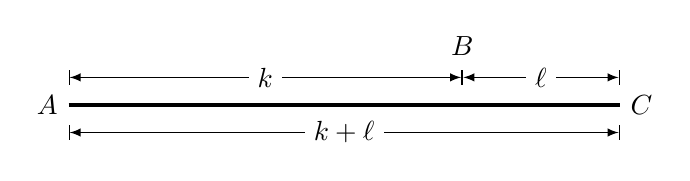
\begin{tikzpicture}[>=latex]
\draw[|<->|] (0,-.35)--node[fill=white]{$k+\ell$}(7,-.35);
\draw[|<->|] (0,.35)--node[fill=white]{$k$}(5,.35);
\draw[|<->|] (5,.35)--node[fill=white]{$\ell$}(7,.35);
\node at (5,.5)[above]{$B$};
\draw[very thick](0,0)node[left]{$A$}--(7,0)node[right]{$C$};

\end{tikzpicture}
    \caption{}
\end{figure}

现在我们定义积$ab$, 如图6.7(1), 画了一个任意角,
在它的一边上,从顶点开始顺次截取长度为1和$b$的线段
$OA$和$AC$, 在另一边上截取长度为$a$的线段$OB$, 此外,作直
线$CD$平行于直线$AB$, $CD$截得的线段$BD$的长度,定义为积
$ab$. 这个定义是合理的,因为如果我们在另一个角$O'$上类似
地作图(图2.7(2)),那么得到的线段$B'D'$的长度和线段
$BD$的长度相等。

\begin{figure}[htp]
    \centering
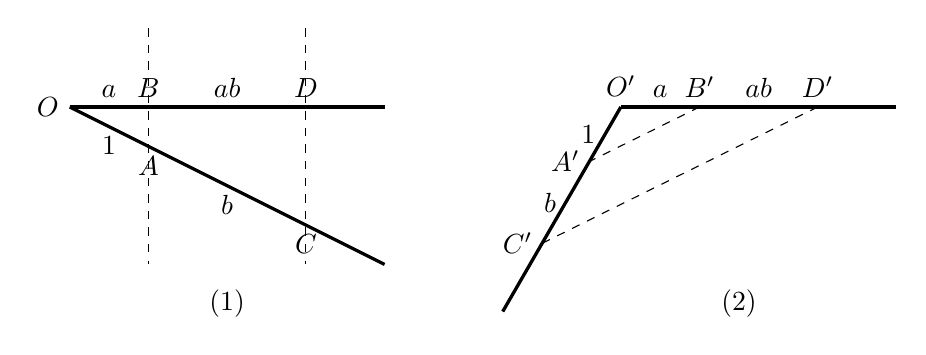
\begin{tikzpicture}[>=latex]
\begin{scope}
    \draw[very thick] (0,0)node[left]{$O$}--(4,0);
    \draw[very thick] (0,0)--(4,-2);
    \draw[dashed] (1,1)--(1,-2);
    \draw[dashed]  (3,1)--(3,-2);
    \foreach \x/\xtext in {1/B,3/D}
    {
        \node at (\x,0) [above]{$\xtext$};
    }
    \foreach \x/\xtext in {1/A,3/C}
    {
        \node at (\x,-.5*\x) [below]{$\xtext$};
    }
\node at (2,-2.5){$(1)$};
\node at (.5,-.25)[below]{1};
\node at (.5,0)[above]{$a$};
\node at (2,-1)[below]{$b$};
\node at (2,0)[above]{$ab$};
\end{scope}
\begin{scope}[xshift=7cm]
    \draw[very thick] (0,0)node[above]{$O'$}--(3.5,0);
    \draw[very thick] (0,0)--(-120:3);
\draw[dashed]  (1,0)node[above]{$B'$}--(-120:.8)node[left]{$A'$};
\draw[dashed]  (2.5,0)node[above]{$D'$}--(-120:2)node[left]{$C'$};
\node at (.5,0)[above]{$a$};
\node at (-120:1.4)[left]{$b$};
\node at (3.5/2,0)[above]{$ab$};
\node at (-120:.4)[left]{$1$};
\node at (1.5,-2.5){$(2)$};
\end{scope}

\end{tikzpicture}
    \caption{}
\end{figure}

除法运算定义为乘法的逆运算。如图6.8, 在角的一边
上从顶点开始,顺次截取长度为$b$和$a$的线段,而在另一边上
截取单位线段,作$CD$平行于$AB$, 于是$AC$的长度定义为$\frac{a}{b}$
这个定义也是合理的,并且$b\left(\frac{a}{b}\right)=a$。

最后,我们来规定负长度和零长度。在数轴上,原点$O$
右边的点和这点与点$O$的连接线段的长度成一一对应,我们
把这种长度称为正的长度。我们把直线上关于原点$O$和点$A$
(即对应长度为$a$的点)对称的点$A'$的相应线段的长度,形
式地规定为负的长度$-a$, 规定点$O$对应于长度零。结果在
整个直线上的点和实数之间建立了一一对应。

现在从几何上容易验证实数在四则运算和大小次序这两
种结构上满足下面的基本性质,例如,用图6.9可以验证分
配律$a(b+c)=ab+ac$。

\begin{figure}[htp]\centering
    \begin{minipage}[t]{0.48\textwidth}
    \centering
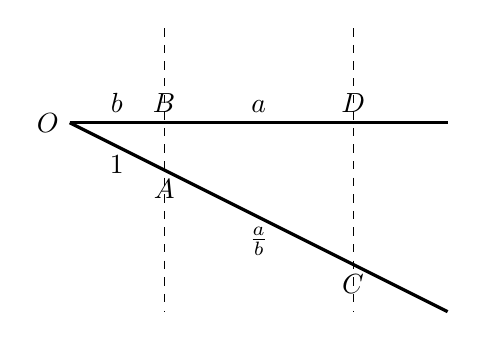
\begin{tikzpicture}[>=latex, scale=1.2]
    \draw[very thick] (0,0)node[left]{$O$}--(4,0);
    \draw[very thick] (0,0)--(4,-2);
    \draw[dashed] (1,1)--(1,-2);
    \draw[dashed]  (3,1)--(3,-2);
    \foreach \x/\xtext in {1/B,3/D}
    {
        \node at (\x,0) [above]{$\xtext$};
    }
    \foreach \x/\xtext in {1/A,3/C}
    {
        \node at (\x,-.5*\x) [below]{$\xtext$};
    }

\node at (.5,-.25)[below]{1};
\node at (.5,0)[above]{$b$};
\node at (2,-1)[below]{$\frac{a}{b}$};
\node at (2,0)[above]{$a$};   
    \end{tikzpicture}
    \caption{}
    \end{minipage}
    \begin{minipage}[t]{0.48\textwidth}
    \centering
    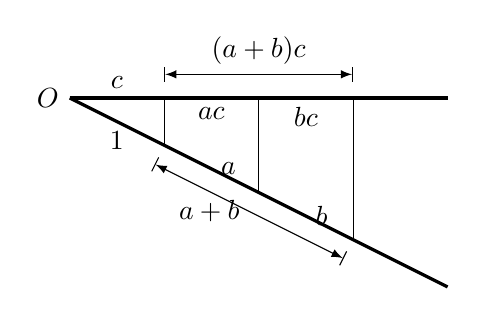
\begin{tikzpicture}[>=latex, scale=1.2]
 \draw[very thick] (0,0)node[left]{$O$}--(4,0);
    \draw[very thick] (0,0)--(4,-2);
    \draw (1,0)--(1,-.5);
    \draw  (2,0)--(2,-1);
    \draw  (3,0)--(3,-1.5);
\node at (.5,-.25)[below]{1};
\node at (.5,0)[above]{$c$};
\node at (1.5,0)[below]{$ac$};   
\node at (2.5,0)[below]{$bc$};   
\node at (1.5,-0.75)[right]{$a$};   
\node at (2.5,-1.25)[right]{$b$};  
\draw[|<->|] (1,.25)--node[above]{$(a+b)c$}(3,.25);
\draw[|<->|] (1-.1,-.5-.2)--node[left]{$a+b$}(3-.1,-1.5-.2);
    \end{tikzpicture}
    \caption{}
    \end{minipage}
    \end{figure}

\subsubsection{加法和乘法的运算性质}

\begin{enumerate}
    \item 交换律:$a+b=b+a;\qquad  ab=ba$
    \item 结合律:$(a+b)+c=a+(b+c);\qquad (a\cdot b)\cdot c=a\cdot (b\cdot c)$
    \item 分配律:$a\cdot (b+c)=a\cdot b+a\cdot c$
   \item 可逆性:$a+x=b;\qquad a\cdot x=b\; (a\ne 0)$都是唯一可解的,第一式的解是$b-a$; 第二式的解是$b/a$。
\end{enumerate}

\subsubsection{顺序性}
\begin{enumerate}
    \item 对于任意实数$a,b$, 下列关系中有一种且仅有一
    种成立:
    \[a>b,\qquad a=b\quad \text{或}\quad a<b\]
    \item 由$a<b$和$b<c$推出$a<c$(符号“$<$”的传递性)。
    \item 设$a<b$则$a+c<b+c$
    \item 符号定则
    \[\begin{cases}
        a>0,\qquad b>0\\
        a>0,\qquad b<0\\
        a<0,\qquad b<0
    \end{cases}\Rightarrow\quad  \begin{cases}
        a\cdot b>0\\a\cdot b<0\\a\cdot b>0\\
    \end{cases}\]
    \item 对于任意两个正实数,$a,b>0$, 恒存有一够大
    的正整数$n$, 使得$na<b$。 (通常称之为阿基米德性质)
\end{enumerate}

\subsubsection{ 实数集连续性(完备性)}
我们已经知道实数系与有理数系在加、乘及不等式的运
算上有完全相同的性质,但是实数系还具有一个有理数系所
没有的优良性质,那就是下面讨论的实数系连续性(完备
性)。

在前面,我们用二分法和十分法为例,说明了任何给
定的实数$x$都可以用有理数去逼近它。我们所用的是两个有
理数列$\{a_n\}$和$\{b_n\}$从左、右夹逼$x$,$\{a_n\}$, $\{b_n\}$和$x$之间的关
系可以用下面这一串次序关系来表达:
\[a_1\le a_2\le\cdots\le a_n\le \cdots <x<\cdots\le b_n\le \cdots\le b_2\le b_1\]
$(b_n-a_n)$可以任意小,记作$(b_n-a_n)\to 0$。上面是实数$x$已经先给定
了的情况,去求出两串数列$\{a_n\}$和$\{b_n\}$来左、右夹逼实数$x$,
也就是说,数轴$\ell$上的每一点,即每一个实数,能够由上述
的两个有理数列来唯一确定。反过来问,假如先给定了满足
下述这样一串大小次序关系的$\{a_n\}$和$\{b_n\}$, 即
\[a_1\le a_2\le\cdots\le a_n\le \cdots \le b_n\le \cdots\le b_2\le b_1\]
且$(b_n-a_n)$可以任意小,是不是会有那么一个实数$x$去被
$\{a_n\}$、$\{b_n\}$左、右夹逼呢?上述问题的答案是肯定的!因为
从实数系在长度度量的直观上看,这个实数$x$的存在也就是
说实数轴上没有空隙存在,即直线是连续不断的,换言之,
实数系也是连续不断的,因此我们称实数系为\textbf{实数连续统};
它说明实数系包含着度量时所有应该包含的数,所以也叫做
实数系的\textbf{完备性}。下面是直线连续不断的直观概念的解析
描述。

\begin{blk}{实数系完备性}
     对于任给满足下述大小次序关系的两个
数列$\{a_n\}$和$\{b_n\}$,即
\[a_1\le a_2\le \cdots a_n\le \cdots \le b_n\le \cdots \le b_2\le b_1\]
且$(b_n-a_n)\to 0$,则必定存在一个介于所有$a_n,b_n$之间的实
数$x$。
\end{blk}


实数系的完备性是非常基本而且重要的!在以后的章节
中,我们将用这个性质来证明极限的存在,从而可进行一切
极限运算,而这些运算乃是微积分的基础。在每次用到时,
我们将详细解说其用法。这样逐步渐近,同学不难学会它的
种种用法。

\section*{习题6.1}
\addcontentsline{toc}{subsection}{习题6.1}

\begin{enumerate}
    \item 证明$\sqrt{3}$是无理数。
    \item 设$\sqrt{5}=a$, $a$的小数部分用$b$表示,求$a-\frac{1}{b}$。
\item 若$a+\sqrt{b}=c+\sqrt{d}$, 这里$a,b,c,d$是有理数而$\sqrt{b}$是无理数,则$a=c$, $b=d$, 试证之。

\item 利用“整系数方程
$a_0x^n+a_1x^{n-1}+\cdots+a_{n-1}x+a_n=0$
的任何有理根,如果写成既约分数时为$\frac{p}{q}$,
那么分子$p$是
$a_n$的约数,分母$q$是$a_0$的约数”,这一准则使我们能够得到一
切有理实根,从而证明任何其它根都是无理数。

试证明:
$3+2\sqrt{2}$, $1+\sqrt[3]{3}$, $\sqrt[3]{2}+\sqrt[3]{4}$都是某一整系数方程
的无理根,从而证明这些数都是无理数。
\item \begin{enumerate}
    \item 如果$a$是有理数,$x$是无理数,试证明$a+x$是无
理数;又如果$a\ne 0$, 试证明$ax$是无理数。
\item 试证明任何两个有理数之间至少存在着一个无理
数,因而存在着无穷多个无理数。
\end{enumerate}

\item 试证明:任给无理数$a$和正整数$m$, 我们可以找到
分数$\frac{n}{m}$,使得$\left|a-\frac{n}{m}\right|<\frac{1}{2m}$
\item 若等腰三角形的顶角为$36^{\circ}$, 底边长为1, 试证它
的腰长不能用有理数表示。
\item 用二分逼近法求下列无理数的有理近似值,使得误
差小于$\frac{1}{100}$:
\begin{multicols}{2}
    \begin{enumerate}
        \item $\sqrt{7}$
        \item $\sqrt[3]{2}$
    \end{enumerate}
\end{multicols}
\end{enumerate}

\section{不等式与绝对值}
不等式在高等数学中所起的作用要比在初等数学中大得
多,一个量$x$的精确值往往难以确定,不过,对$x$进行估值,
即指明$x$大于某个已知量$a$而小于另一个已知量$b$, 却是容
易做到的。在许多应用中,重要的只是知道$x$的这种估值。
为以后学习方便起见,我们要在这一节比较详细地回顾一下
不等式的一些重要性质。

\subsection{不等式的性质}
$a$和$b$是实数,如果$a-b>0$, 那么就称$a$大于$b$, 记作
$a>b$; 如果$a-b<0$, 那么就称$a$小于$b$, 记作$a<b$; 如
果$a-b=0$那么就称$a$等于$b$, 记作$a=b$. 注意若$a<b$有
时也说成$b>a$, 因此$a<b$和$b>a$是等价的。

应用两个正实数之和或积仍然是正数这个基本事实,即
如果$a>0$和$b>0$则有$a+b>0$和$ab>0$, 而且依据不等式$a>b$
等价于$a-b>0$, 我们容易推导出下面的性质。

\begin{blk}{性质1}
    若$a>b$和$c>d$, 则$a+c>b+d$。换言之,同向
的两个不等式可以相加。
\end{blk}

\begin{blk}{性质2}
    若$a>b$且$c>0$, 则$ac>bc$。
\end{blk}

\begin{blk}{性质3}
    若$a>b$且$c<0$, 则$ac<bc$。
\end{blk}

上面的性质2和性质3也可以表达为不等式若乘以正数得到
同向不等式;若乘以负数则得到异向的不等式。更一般地可
以得到:

若$a>b>0$和$c>d>0$则$ac>bd$。
也就是两个同向的正数不等式可以相乘。


\begin{blk}{性质4}
    \begin{itemize}
        \item 若$a>b>0$, 则$\frac{1}{a}<\frac{1}{b}$;
        \item 若$a>0>b$, 则$\frac{1}{a}>0>\frac{1}{b}$;
        \item 若$a<b<0$, 则$\frac{1}{a}>\frac{1}{b}$。
    \end{itemize}
 \end{blk}   

\begin{blk}{性质5}
    若$a>b$而$b>c$, 则$a>c$。
\end{blk}

这就是说不等式具有传递性,在几何上这是显然的,也可由
 $(a-b)+(b-c)=a-c$为正直接推出,在上述推演中,如果
 我们处处都用符号$\ge $代替$>$,则各项法则仍然成立。

\begin{blk}{性质6}
    若$a>b>0$, 则$a^2>b^2$。
\end{blk}

我们注意到$a^2-b^2=(a+b)(a-b)$, 因为$a+b$是正数,
 由$a>b$可以推出,$a^2>b^2$. 这样正数之间不等式可以进行平
 方运算。

\begin{blk}{性质7}
    若$a>b>0$, 则$\sqrt{a}>\sqrt{b}$,
 即在正实数之间的不等式两端能取平方根。
\end{blk}

事实上,$\sqrt{a}-\sqrt{b}=\frac{a-b}{\sqrt{a}+\sqrt{b}}$
,因为$\sqrt{a}+\sqrt{b}$是
正数,从而由$a>b$就可推出$\sqrt{a}-\sqrt{b}>0$, 即$\sqrt{a}>\sqrt{b}$。

更一般地,若$a>b>0$ 且$n$是自然数,那么
$a^n>b^n$。

这个结论可以用数学归纳法来证明。这个证明留给同学作为
练习。

反过来,若$a>b>0$, 且$n$是一个正整数,则$a^{\tfrac{1}{n}}>b^{\tfrac{1}{n}}$。

\begin{proof}
    假设$a^{\tfrac{1}{n}}=b^{\tfrac{1}{n}}$, 那么$\left(a^{\tfrac{1}{n}}\right)^n>\left(b^{\tfrac{1}{n}}\right)^n$,因而,$a=b$, 这就与已知$a>b$矛盾。

假设$a^{\tfrac{1}{n}}<b^{\tfrac{1}{n}}$, 于是$\left(a^{\tfrac{1}{n}}\right)^n<\left(b^{\tfrac{1}{n}}\right)^n$,即$a<b$, 这又与已知
条件$a>b>0$矛盾,故我们得出结论$a^{\tfrac{1}{n}}>b^{\tfrac{1}{n}}$。
\end{proof}


\subsection{绝对值不等式}
我们回想到$|x|$的定义是这样的:

\begin{blk}{定义}
$x$是一个实数,当$x$是一个非负数时,$x$的绝对
值$|x|$是它本身;当$x$是一个负数时,$x$的绝对值$|x|$是$x$
的相反数。



\end{blk}









\begin{example}
    
\end{example}


\begin{solution}
    
\end{solution}

\begin{example}
    
\end{example}

\begin{solution}
    
\end{solution}


\begin{example}
    
\end{example}

\begin{example}
    
\end{example}

\begin{solution}
    
\end{solution}

\begin{solution}
    
\end{solution}

\begin{example}
    
\end{example}

\begin{example}
    
\end{example}

\begin{example}
    
\end{example}

\begin{example}
    
\end{example}

\begin{example}
    
\end{example}

\begin{example}
    
\end{example}

